	\chapter{Expected Outcomes}
    	The labelling system works properly. Sentences from the database were properly displayed in the web application. Labeler successfully labelled about 5,680 data points which was stored in 512KB chunks of files. The system for labelling Nepali sentiment sentences has been completed. The input data from the file was successfully retrieved, then preprocessed and sent to the model for training.
    	\vspace{0.2in}
    	Various models for sentiment classification was trained and the results of the training are shown in the table below:
    	
\begin{center}
    \begin{tabular}{|p{1cm}|p{3cm}|p{4cm}|p{4cm}|p{2cm}| }
        \hline
        S.N. & Model & Training Accuracy & Testing Accuracy & Epochs\\
        \hline
        1. & LSTM RNN Model & 80\% & 82\% & 3\\
        \hline
        2. & Attention Based LSTM RNN & 88\% & 80\% & 5 \\
        \hline
        3. & POS integrated LSTM RNN & 86\% & 74.5\% & 4 \\
        \hline
        4. & Attention based POS integrated LSTM RNN  & 89\% & 75\% & 4 \\
        \hline
    \end{tabular}
    \begin{figure}[h]
	    \centering
		    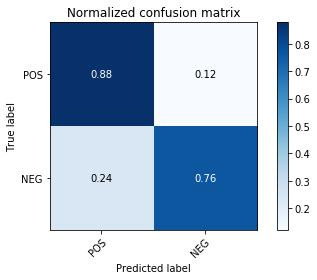
\includegraphics[width=0.75\textwidth]{./img/7.1.jpg}
		    \caption{Confusion matrix for LSTM RNN Model}
	\end{figure}
\end{center}	
	The best model was found to be LSTM RNN Model with testing accuracy 82\%, recall 87\%, precision of 76\%. Other models performed worse than this model was due to added complexity for low datapoints. After building the basic LSTM model we tried to 
	increase its accuracy by changing various variables such as changing word embedding, adding POS feature to the basic model but, due to low number of datapoints for added complexity in the model, they started overfitting. To solve the problem of overfitting of the model we tried different measures such as dropout, regularization and increasing data. But increasing data was not an option for us due to limited time.\\\\
	increase its accuracy by changing various variables such as changing word embedding, adding POS feature to the basic model but, due to low number of datapoints for added complexity in the model, they started overfitting. To solve the problem of overfitting of the model we tried different measures such as dropout, regularization and increasing data. But increasing data was not an option for us due to limited time.